\section{Components}
We have split the different functionality that the final bus needs into four components, that we can design, implement and test separately. We go through these components in this section. Additionally, we will test these using tracks designed specifically to decide whether the components conform to the requirements \ref{Requirements}.

%This section lists the different prototypes with their design, purpose, and objectives that it needs to fulfil in order to be a completed prototype. Furthermore, it will describe the tracks that are designed for testing the functionality of each prototype. The prototypes will take base from the requirements in section \ref{Requirements}.


\subsection{Staying Within the Lines}

\subsubsection{Component Requirements}
The requirements for this component are a reduced amount of the total requirements for the project.

From requirement 1, the component must be able to navigate a track constructed with the same relation between its width and the width of the bus as the \todo{Nej er først prototype.2}Danish Road Directorate dictates for Danish roads. This means the bus needs to drive, brake and turn. The bus' maximum turning radius only needs to be at least as much as the maximally allowed curve on Danish roads. 

As a less demanding requirement 4, the first component should avoid collisions with obstacles from the front. \unsure{The second requirement isn't strictly part of the steering "component", instead it's part of the overall bus prototype}

\subsection{Prototype Construction}
To create the component focused on steering the bus through the track, which will later be used in the final product, a prototype designed solely for this purpose is built. The prototype needs to be able to drive, turn and brake. Furthermore, it needs to be able to combine these mechanisms to stay within the lines of the track. A LEGO Servo Motor is connected to the rear wheels, which provides forwards and backwards movement capabilities. The speed consistency of the bus is not important in this prototype, however driving at a higher speed allows for testing the capabilities of the sensors and their processing speed.
%however the Servo Motor should be set at \todo{80\%}, to make sure the bus can drive at high speed and still stay within the lines at all times, but the actual speed are not to be measured.

\textbf{Turning}\newline
The front wheels are used for turning and is powered by a LEGO Servo Motor. It should be able to turn the same amount of degrees to both sides, however, there is no requirement for a specific turning angle for this prototype. A thing to note is that the track for the bus should be designed such that the bus can perform the turn within the lines.

\textbf{Obstacle Detection}\newline
To prevent crashes, the prototype supports obstacle detection by having a LEGO ultrasonic sensor mounted at the very front of the bus in a fixed position. The sensor detects obstacles up to 70 cm ahead and 30 degrees to both sides. If it predicts that a collision might occur, the bus stops immediately, overriding both the driving and turning procedures. When the obstacle is no longer a hindrance, it will return to its normal state.  % Later prototype should be able to get out of this situation

\textbf{Follow Track}\newline
For the prototype to stay within the lines of the track, a LEGO NXTCam-v4 should be placed at the front in the center. The sensor should be aimed at the ground in front of the bus in order to see the tracks.

The bus itself should be formed like a long rectangle so that it gets the form of a bus. It should have \todo{1:3?} length to width ratio.

\subsubsection{Track requirements}
The designed track for this prototype can be seen in figure \ref{Track1Layout}. The layout of the track is quite simple and only contain some of the requirements described in section \ref{Requirements}. The reason for this is to only test the features of this prototype and as such, it is designed uniquely for this prototype.

The requirements for the track has therefore been limited to:
\cite{DriveingCurves}
\begin{itemize}
  \item One lane, with a width of the minimal turning space requirement.
  \item 6\% extra lane width on each side.
  \item 180 degrees turn with the minimal length and width.
  \item A Small turn.
  \item Pedestrian crossing for testing obstacle detection.
\end{itemize}

\begin{figure}[H]
    \label{Track1Layout}
    \centering
    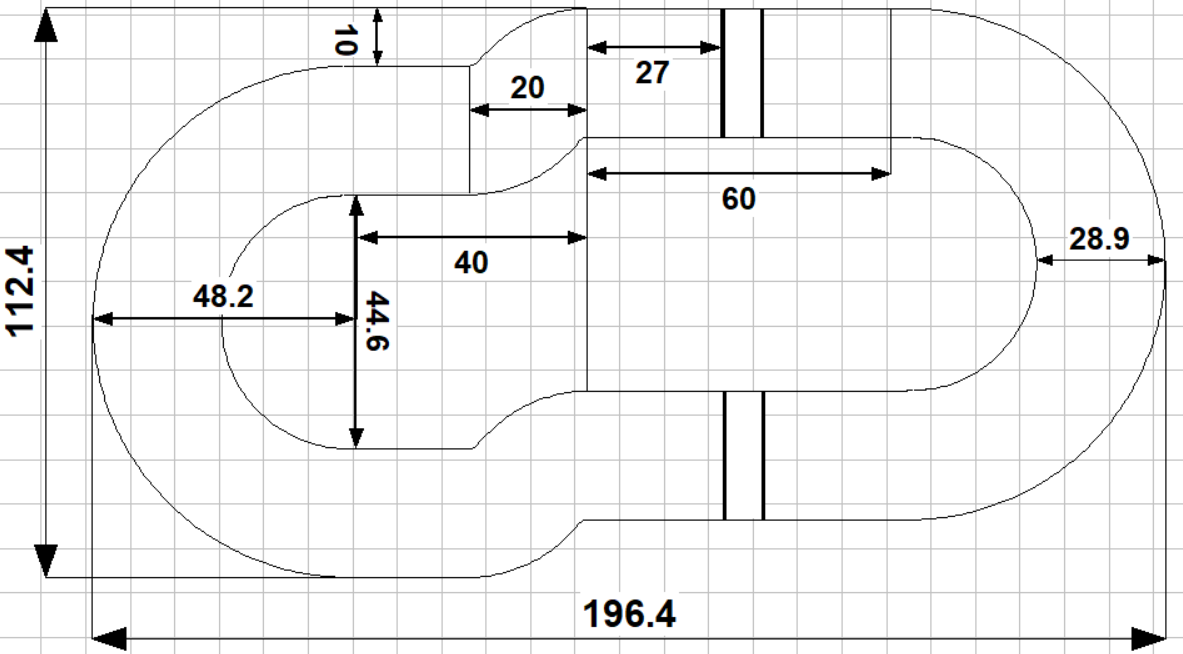
\includegraphics[width=0.8\textwidth]{Images/Tracks/Track1.PNG}
    \caption{Track 1 Layout in cm}
\end{figure}

\todo{Insert Final layout}








%\subsection{2. Prototype - Bus stop procedure}
%The second component is focused on detecting and performing a bus stop, and is built using the component of the steering object. 

%Using the requirements, this component needs to:\\
%    - Detect Bus Stops\\
%    - Stop parallel to the curb\\
%    - Stop within 1 cm of the curb

%The track will need to have some bus stops build on it, and it will also need to have some way to signal to the bus that a bus stop is coming up. This will most likely be a coloured piece of tape, that the bus will recognise with a LEGO colour sensor.\info{This is at least the plan as of this moment.}  Furthermore the track will also have to be circular to allow for the bus to keep driving around on the track and make repeated stops at the bus stops.



\subsection{2. Iteration - Bus stop procedure \& Speed Controller}
Intro: beskriv curb/bus stop procedure


\textbf{Bus stop procedure} \newline

\textbf{Speed Controller} \newline


\textbf{Track requirements} \newline
The redesigned track for the second iteration can be seen on figure.\todo{some stuff to fix here} %\ref{Track2Layout}.
The track is quite similar to the first track, however in this iteration the track contains a bus stop, and is connected so it's infinite. Furthermore the aspect ratio have been changed slightly to fit the redesigned bus, that means the minimal turning radius and lane width have been recalculated as described in appendix \ref{laneCalculations}. Lastly the track contains three new tape colours placed between the two lane tapes. The three colours are to be used with the nxt color sensor to detect incoming bus stops, and to determine the speed limit of the road.

The new requirements for the track is therefore as follows:
\begin{itemize}
  \item Detect Bus Stops
  \item Stop parallel to the curb(tape)
  \item Stop within 1 cm of the curb(tape)
  \item Stop so the bus sign is 1cm from the right corner of the bus
  \item Red tape to illustrate an incoming bus stop
  \item Green tape to illustrate high speed zone(Major Highway)
  \item Blue tape to illustrate low speed zone(Street)
\end{itemize}

\begin{figure}[H]
    \label{Track2Layout}
    \centering
    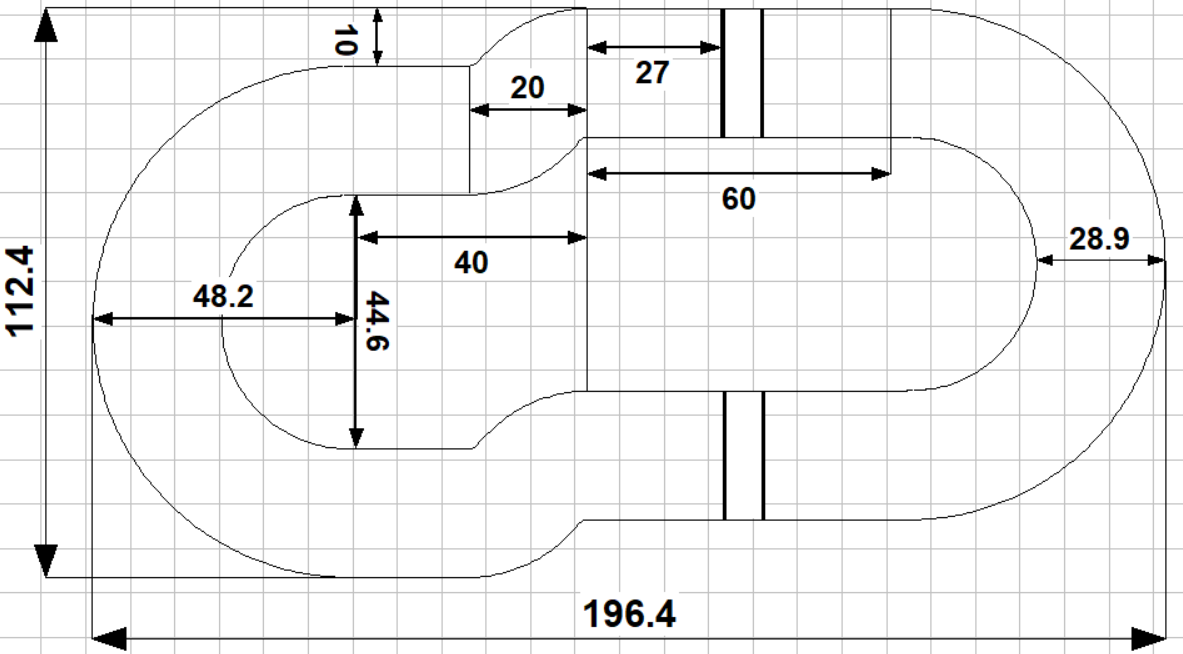
\includegraphics[width=0.8\textwidth]{Images/Tracks/Track1.PNG}
    \caption{Track 2 Layout in cm}
\end{figure}

\textbf{Bus Reconstruction} \newline
The redesigned bus can be seen on figure \ref{busDesign2}\todo{Missing picture of bus to reference}. The bus was redesigned to fix a couple of issues which was found upon testing in the first iteration.

\begin{itemize}
  \item Rear wheels felt off after the bus had driven for some time
  \item Unbalanced weight, which made it hard for the bus to turn left, but not right.
  \item The width and depth of the bus was not consistent, e.g. the ultrasonic sensor was placed too far in front. 

\end{itemize}

insert billede.












%OLD:
%As previously mentioned
%\ref{solvingRequirements
%\todo{fix}, we intend wish to detect a physical object emulating a sign and not just a drawing on the tracks. Towards this end we will be attempting to use a NXT CamV4 Sensor and some image recognition algorithm. 


%The bus scale should be a close approximate of a real bus scale as \cite{DriveingCurves}, 
\subsection{3. Prototype - Cruise Control, BT stop button, obstacle safety protocol}
\subsection{4. Prototype - Detecting bus stops}